\documentclass[10pt]{article}
\usepackage[utf8]{inputenc}
\usepackage[spanish]{babel}
\usepackage{amsmath}
\usepackage{amsfonts}
\usepackage{amssymb}
\usepackage{graphics}
\usepackage{graphicx}
\usepackage[left=2cm,right=2cm,top=2cm,bottom=2cm]{geometry}
\usepackage{imakeidx}
\makeindex[columns=3, title=Alphabetical Index, intoc]
\usepackage{listings}
\usepackage{multicol}
\usepackage{changepage}
\usepackage{float}
\usepackage{cite}
\usepackage{url}
\usepackage{hyperref}
\usepackage{pdflscape}
\usepackage[document]{ragged2e}
\usepackage{xcolor,colortbl}

\hypersetup{
    colorlinks=true,
    linkcolor=blue,
    filecolor=magenta,
    urlcolor=blue,
}

\definecolor{Red}{rgb}{0.7,0,0}
\definecolor{LightCyan}{rgb}{0.88,1,1}
\definecolor{AquaCyan}{rgb}{0.2,1,0.5}
\definecolor{Gray}{gray}{0.85}
\definecolor{DarkBlue}{rgb}{0.1,0.1,0.5}

\definecolor{codegreen}{rgb}{0,0.6,0}
\definecolor{codegray}{rgb}{0.5,0.5,0.5}
\definecolor{codepurple}{rgb}{0.58,0,0.82}
\definecolor{backcolour}{rgb}{0.95,0.95,0.92}

\lstdefinestyle{mystyle}{
    backgroundcolor=\color{backcolour},
    commentstyle=\color{codegreen},
    keywordstyle=\color{magenta},
    numberstyle=\tiny\color{codegray},
    stringstyle=\color{codepurple},
    basicstyle=\ttfamily\footnotesize,
    breakatwhitespace=false,
    breaklines=true,
    captionpos=b,
    keepspaces=true,
    numbers=left,
    numbersep=5pt,
    showspaces=false,
    showstringspaces=false,
    showtabs=false,
    tabsize=3
}
\def\fillandplacepagenumber{%
 \par\pagestyle{empty}%
 \vbox to 0pt{\vss}\vfill
 \vbox to 0pt{\baselineskip0pt
   \hbox to\linewidth{\hss}%
   \baselineskip\footskip
   \hbox to\linewidth{%
     \hfil\thepage\hfil}\vss}}
\lstset{style=mystyle}

\title{Centro de Investigación en Cómputo\\Instituto Politécnico Nacional\\Metaheurísticas\\Actividad 19: Solución de problemas mediante heurísticas de trayectoria simple y evolutivas\\Curso impartido por: Dra Yenny Villuendas Rey}

\author{Adrian González Pardo}

\date{\today}

\newcommand\tab[1][1cm]{\hspace*{#1}}

\begin{document}
\maketitle
\section{Heurísticas}
\subsection{Random Mutation Hill Climbing Algorithm (RMHC)}
Es un algoritmo heurístico de trayectoria simple, es decir, que la solución a buscar o a obtener es dada por un estado inicial y a partir de el se realiza la exploración del área en búsqueda de un óptimo global o local, por ello:
\begin{center}
  \begin{tabular}{|p{5cm}|p{5cm}|}
    \hline
    Ventajas & Desventajas \\
    \hline
    Permite realizar un número menor de iteraciones con respecto a la exploración del espacio en modalidad de fuerza bruta & El resultado puede quedarse en un mínimo local sin que sea el mínimo del espacio\\
    \hline
    Permite moverse en el espacio de diferentes formas, permitiendo que encuentre un mínimo & Dependiendo de la implementación del algoritmo puede que que llegue al mínimo o no, pero al final arroja una solución \\
    \hline
    Dependiendo de la implementación puede que tenga un número distinto de iteraciones & En caso de ser un espacio muy grande puede que la implementación, salto o movimiento entre el espacio demore demasiado\\
    \hline
  \end{tabular}
\end{center}
Una vez explicado las ventajas y desventajas se trata de un algoritmo que actúa a partir de una solución aleatoria la cual al obtener un valor aleatorio $m$ este puede representar una cadena de bits sobre la cual puede interpretarse como una mutación real de un arreglo vía índice o como una mutación de bits la cual intercambiara los valores de diversas áreas de un arreglo o que permutara, todo depende de la implementación, a partir de el se buscara o se desea que la modificación de la respuesta inicial sea más óptima o aproximada a la solución determinista del programa.
\subsection{Simulated Annealing Algorithm (SA)}
Al igual que RMHC esta es una heurística de trayectoria simple que a diferencia del mismo RMHC, esta permite aceptar o escapar de un óptimo local, con la idea de llegar al óptimo global, por ello:
\begin{center}
  \begin{tabular}{|p{5cm}|p{5cm}|}
    \hline
    Ventajas & Desventajas \\
    \hline
    Permite obtener una solución aproximada al mínimo global & Puede llegar a pasar que en la siguiente iteración del programa, esta salga del mínimo global y este se alcance un resultado mínimo local o en otra área\\
    \hline
    Permite encontrar soluciones razonables (En tiempo) & La solución encontrada puede no ser la mejor\\
    \hline
    Utiliza poca memoria & No permite vuelta atrás en más de 1 paso\\
    \hline
  \end{tabular}
\end{center}

Este tipo de heurística busca simular el enfriado de metales por ello en el algoritmo se implementa una temperatura máxima a la cual el algoritmo comenzara a trabajar, más tarde después de ello se enfriara mediante un factor $\alpha$ el cual puede ser seleccionado aleatoriamente en el intervalo de $[0,1]$ de modo que en el trabajo presente el intervalo fue modificado para que $\alpha$ tome un valor aleatorio desde $[0.88,0.99]$ de modo en que este llegue o converja en una solución óptima.
\subsection{Genetic Algorithm (GA)}
A diferencia de las dos heurísticas previas que funcionan como trayectoria simple, esta heurística es un algoritmo o un modelo poblacional en el cual se busca generar múltiples soluciones las cuales competirán por ser seleccionadas mediante su operador distintivo el cual puede ser una selección por su función, en el que se buscara dos óptimos, para más tarde pasar a través de una función de probabilidad la cual nos indicara si las dos soluciones pueden ser mutadas (modificadas), y después más tarde pueden ser modificadas para formar parte del espacio de solución o de la generación espacial de soluciones, por ello:
\begin{center}
  \begin{tabular}{|p{6cm}|p{6cm}|}
    \hline
    Ventajas & Desventajas \\
    \hline
    Permite realizar múltiples búsqueda de soluciones a los problemas & Puede que el método de mutación o cruza seleccionado puede que no ayude a encontrar una buena solución\\
    \hline
    Esta bioinspirado en la genética y en la selección natural (Darwinismo) & Puede que el que en la aplicación en alguna etapa del GA ya no avance \\
    \hline
    Es una heurística poblacional & Puede que genere bastante uso de recursos en memoria y procesamiento \\
    \hline
    Es posible el trabajar soluciones de formas paralelizables o distribuidas&Puede ser difícil de implementar\\
    \hline
  \end{tabular}
\end{center}
\section{Aplicaciones}
A partir de cualquier heurística se puede realizar o buscar la solución a problemas de la clase \textit{NP-Completo} los cuales pueden se mapeados entre ellos con diversas restricciones, para solucionar y encontrar una función o espacio óptimo de la solución, por ello los principales problemas implementados fueron y han sido Knapsack Problem, Travel Salesman Problem y Minimization Functions (diversas funciones de múltiples variables)
\section{Funciones a optimizar}
\begin{center}
  \begin{tabular}{|c|c|}
    \hline
    Función a evaluar & Forma o descripción de la función\\
    \hline
    Alpine Function & \(\displaystyle f_{1}(x)=\sum_{i=1}^{D} \left|x_{i}\sin(x_{i})+0.1x_{i}\right|\) \\
    \hline
    Dixon \& Price Function & \(\displaystyle f_{2}(x)=(x_{1}-1)^{2}\sum_{i=2}^{D} i\left(2\sin(x_{i})-x_{i-1}\right)^{2}\)\\
    \hline
    Quintic Function & \(\displaystyle f_{3}(x)=\sum_{i=1}^{D} \left|x_{i}^{5}-3x_{i}^{4}+4x_{i}^3-2x_{i}^{2}-10x_{i}-4\right|\)\\
    \hline
    Schwefel 2.23 Function & \(\displaystyle f_{4}(x)=\sum_{i=1}^{D}x_{i}^{10}\)\\
    \hline
    Streched V Sine Wave Function & \(\displaystyle f_{5}(x)=\sum_{i=1}^{D-1}(x_{i+1}^{2}+x_{i}^{2})^{0.25}\left[\sin^{2}\left\{50(x_{i+1}^{2}+x_{i}^{2})^{0.1}\right\}+1\right]\)\\
    \hline
    Sum Squares Function & \(\displaystyle f_{6}(x)=\sum_{i=1}^{D}ix_{i}^{2}\)\\
    \hline
  \end{tabular}
\end{center}
\section{Características de Hardware}
\begin{itemize}
  \item Procesador Intel Core i5-3210M CPU 2.50GHz
  \item Memoria RAM DDR3 12 GB
  \item Sistema Operativo Fedora 32 x86\_64
  \item Ruby 2.7.2p137 para la ejecución
\end{itemize}
\section{Características de ejecución:}
\begin{itemize}
  \item Para las tres heurísticas:
  \begin{itemize}
    \item Dimensiones de la función $10$ y $30$
    \item Máximo número de iteraciones $500$
    \item En la ejecución de operadores normales $\left[-10,10\right]\in\mathbb{R}$
    \item En la ejecución operadores convenientes:
    \begin{itemize}
      \item Quintic con intervalos $\left[2.47,2.479\right]\in\mathbb{R}$
      \item Resto de funciones con intervalos \(\displaystyle\left[ \frac{-10}{random(8\cdots40)}, \frac{10}{random(8\cdots30)} \right]\in\mathbb{R}\)
    \end{itemize}
  \end{itemize}
  \item Para SA:
  \begin{itemize}
    \item Temperatura máxima de $1000$
    \item $\alpha$ aleatorio para cada ejecución del intervalo $[0.88,0.99]$
    \item Temperatura mínima de $0.01$
  \end{itemize}
  \item Para GA ambas implementaciones:
  \begin{itemize}
    \item Población de $10$
    \item Probabilidad de entrar a la mutación $0.5$
    \item Probabilidad de mutar $0.15$
    \item Operador de selección por torneo
    \item Operador de mutación real
    \item Operador de cruzamiento aritmético
    \item Operador de remplazo por elitismo
  \end{itemize}
\end{itemize}
\begin{landscape}
  \section{Tabla de resultados}
  \subsection{Tabla con operadores normales}
  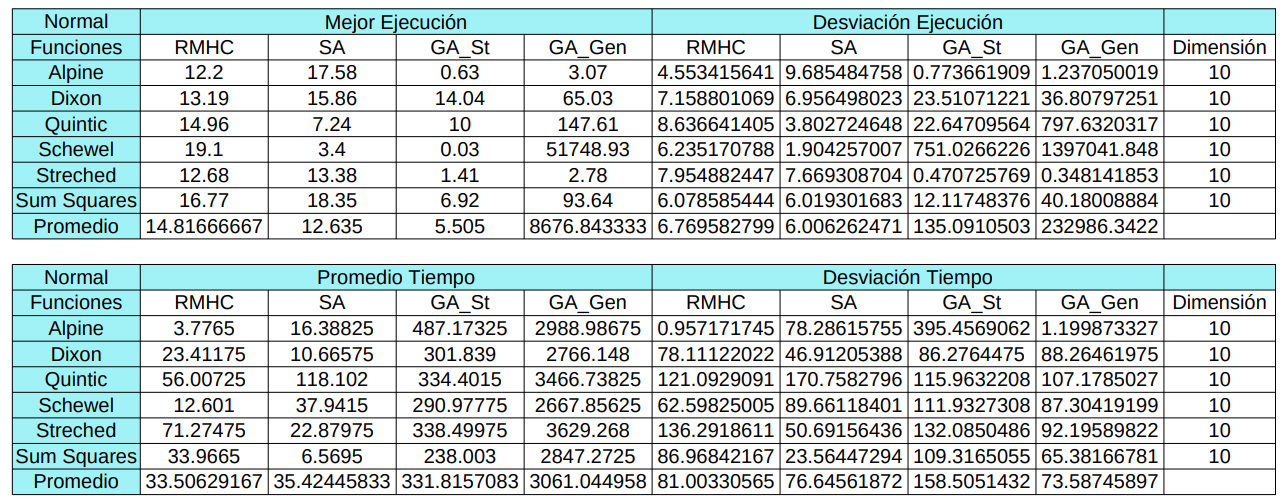
\includegraphics[scale=0.5]{imgs/tabla_1.png}\\
  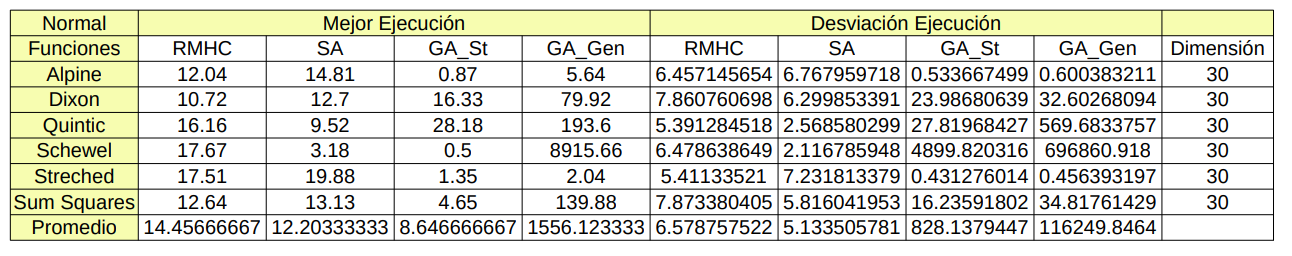
\includegraphics[scale=0.5]{imgs/tabla_2.png}
  \fillandplacepagenumber
  \clearpage
  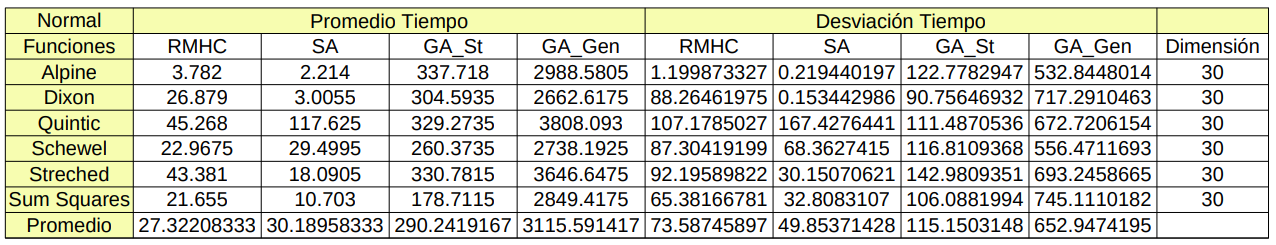
\includegraphics[scale=0.5]{imgs/tabla_3.png}
  \subsection{Tabla con operadores convenientes}
  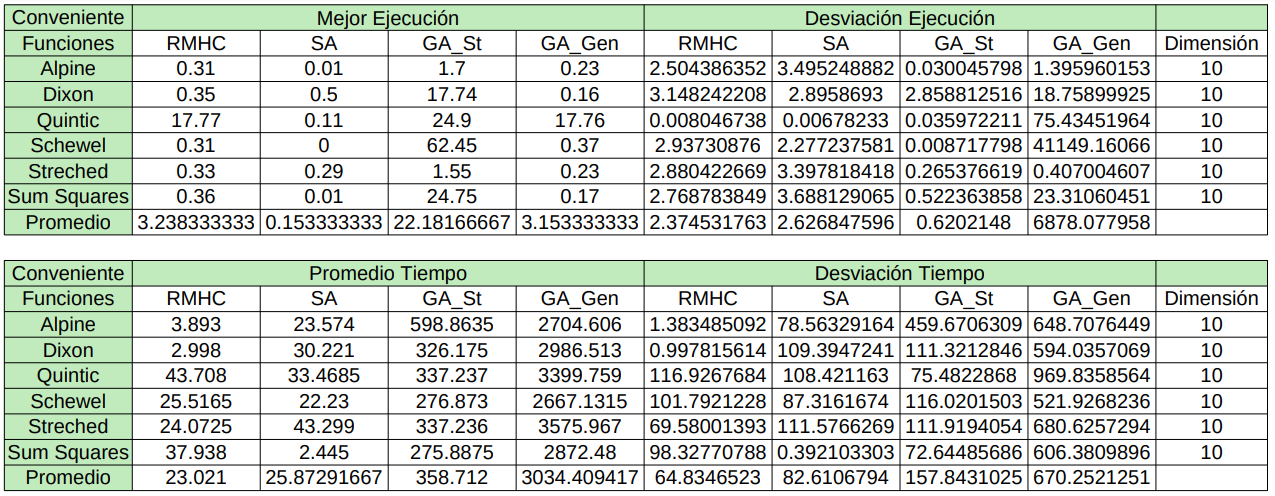
\includegraphics[scale=0.5]{imgs/tabla_4.png}
  \fillandplacepagenumber
  \clearpage
  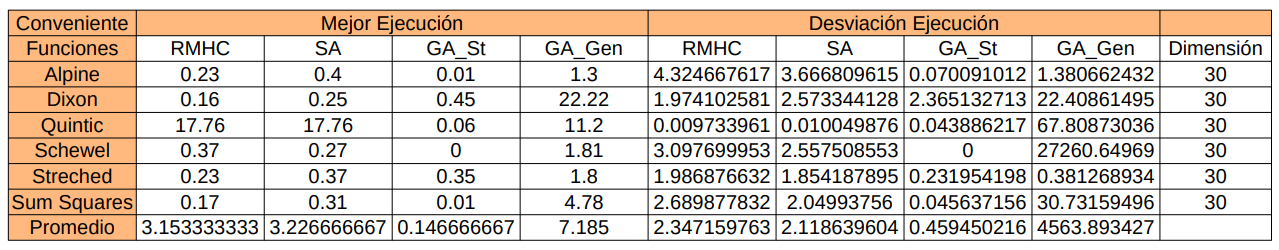
\includegraphics[scale=0.5]{imgs/tabla_5.png}\\
  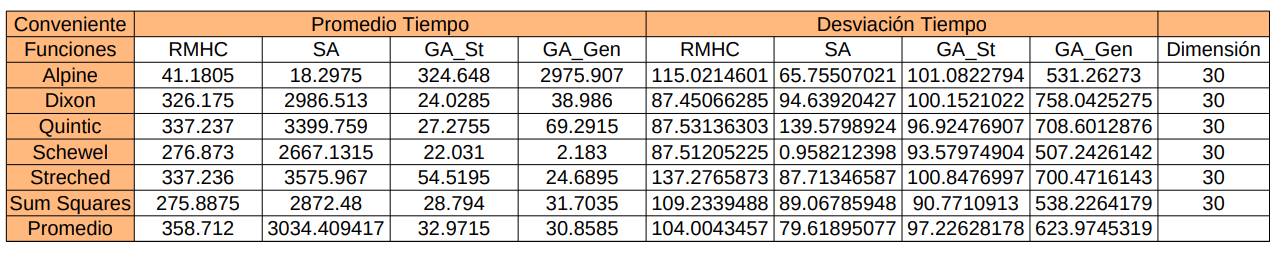
\includegraphics[scale=0.5]{imgs/tabla_6.png}
  \section{Conclusiones}
  Si bien la implementación y comparación de las dos distintas ejecuciones del programa, en este caso relacionadas con realizar las heurísticas mediante intervalos no conocidos de la función, es decir, que van de $[-10,10]$ contra los intervalos más cercanos a la solución del óptimo, nos podemos dar cuenta que no solo infiere mucho el hardware sino también las capacidades de la maquina ya que para la solución en tiempo óptimo de cada heurística fue necesario implementar un pequeño paralelismo el cual permitiera reducir el costo temporal de ejecución de todas y cada una de las heurísticas, para trabajos futuros podría pensarse en una hibridación de las heurísticas para que estas alcancen en su totalidad el óptimo global sin necesidad de utilizar algunos atajos, para llegar a un óptimo local.

  \fillandplacepagenumber
\end{landscape}

\end{document}
